\documentclass[review]{elsarticle}
\usepackage{amsmath,amssymb,amsfonts,amsthm}
\usepackage{booktabs,multirow,array}
\usepackage{graphicx,subcaption}
\usepackage{hyperref,cleveref}
\usepackage{algorithm,algpseudocode}
\usepackage{xcolor,enumitem}

\newtheorem{definition}{Definition}
\newtheorem{proposition}{Proposition}
\DeclareMathOperator*{\softmax}{softmax}
\DeclareMathOperator*{\diag}{diag}

\journal{Cognitive Systems Research}

\begin{document}

\begin{frontmatter}

\title{Adaptive Cognitive Memory Engine: Unifying Multi-Perspective Recall,
Preference Modulation, and Basis Function Evolution via Replicator Dynamics}

\author[1]{Ziheng Pan\corref{cor1}}
\ead{panziheng@aliyun.com}

\address[1]{Independent Researcher}

\cortext[cor1]{Corresponding author.}

\begin{abstract}
We present the Adaptive Cognitive Memory Engine (ACME), a cognitive architecture
that treats memory as spectral compression over interpretable basis functions and
unifies six traditionally independent modules---question routing, preference
modulation, spectrum updating, basis function evolution, safety monitoring, and
intrinsic exploration---through a single replicator dynamics equation.
Facts are encoded as projection coefficients onto ten cognitive dimensions
(causality, emotion, motivation, etc.). The same stored fact yields
qualitatively different reconstructions under different questions or user
preference profiles, because query-dependent filter weights selectively
activate subsets of the spectrum. Basis functions themselves act as strategic
agents in a multi-level evolutionary game, undergoing birth, death, split,
merge, and mutation. Safety constraints are injected as payoff penalties rather
than requiring a separate output-filtering module. Evaluated on a production LLM
across eleven capability dimensions, ACME demonstrates: multi-perspective recall
(attention shift of 0.275$\to$0.378 across query types), feedback-driven spectrum
correction (all 5 basis dimensions updated per feedback signal), spontaneous
population evolution (a new cognitive dimension born via crossover), cross-memory
analogical reasoning (cosine similarity 0.903), and neural-symbolic alignment
(LLM attends to causality 2.1$\times$ more than predicted). We argue that ACME
instantiates a broader design principle: complex adaptive cognitive behavior
emerges from a well-designed fitness landscape rather than independently
engineered modules.
\end{abstract}

\begin{keyword}
Cognitive architecture \sep Memory-augmented AI \sep Replicator dynamics
\sep Concept bottleneck models \sep Evolutionary game theory
\sep Interpretable AI \sep Spectral memory representation
\end{keyword}

\end{frontmatter}

%============================================================
\section{Introduction}
%============================================================

Contemporary large language models (LLMs) exhibit remarkable generative
capabilities~\cite{bommasani2021opportunities}, yet their internal memory
mechanisms remain opaque. When an LLM ``remembers'' a user-provided fact
through in-context learning or fine-tuning, the information is distributed
across billions of weight parameters in a form that is neither inspectable
at the granularity of individual facts, nor editable without retraining,
nor transferable between model instances~\cite{bender2021dangers}.

A parallel line of work on memory-augmented neural networks~\cite{graves2014neural,
graves2016hybrid,weston2014memory} and retrieval-augmented generation
(RAG)~\cite{lewis2020retrieval,karpukhin2020dense} addresses storage by
maintaining explicit external knowledge bases. However, these systems store
and retrieve raw text or dense vector embeddings, lacking a principled
mechanism for extracting different \emph{interpretive perspectives} from
the same stored facts. More recent efforts on personal memory systems such
as Mem0~\cite{mem0} extract structured facts from conversations but treat
memory as a flat key-value store without multi-dimensional cognitive structure.

We identify three fundamental limitations in existing approaches:
\begin{enumerate}[leftmargin=*,itemsep=0pt]
\item \textbf{Single-perspective retrieval.} A stored fact is retrieved as-is
  or via embedding similarity, without the ability to selectively activate
  different semantic dimensions of the same memory.
\item \textbf{Static knowledge organization.} The categories or dimensions
  used to organize memories are predefined and immutable. They do not
  adapt to user behavior or evolve over time.
\item \textbf{Modular complexity.} Systems that attempt to address the
  above limitations typically do so by adding independent modules
  (routers, rankers, filters, moderators), leading to engineering
  complexity and emergent incompatibilities between components.
\end{enumerate}

We propose a different route: an externalized cognitive memory layer in which
facts are stored not as text, but as \textbf{spectral coefficients} over a
finite set of interpretable \textbf{cognitive basis functions}. Crucially,
\textit{all} cognitive operations---routing, modulation, updating, evolution,
safety, and exploration---are derived from a single replicator dynamics
equation~\cite{taylor1978evolutionary,hofbauer1998evolutionary} rather than
implemented as separate modules.

Our contributions are:
\begin{enumerate}[leftmargin=*,itemsep=0pt]
\item \textbf{Spectral memory representation.} We formalize memory as
  projection coefficients onto interpretable cognitive dimensions
  (Definition~\ref{def:spectrum}), unifying compression (10--100$\times$ vs.\
  raw text) with multi-perspective retrieval from a single representation.
\item \textbf{Unified replicator dynamics kernel.} We show that six
  traditionally independent modules emerge as boundary conditions of
  $\dot{x}_i = x_i(\pi_i - \bar{\pi}) + \sum_j(x_j Q_{ji} - x_i Q_{ij})
  + \mu \cdot \text{Mutation}(x_i)$ (Section~\ref{sec:unified}).
\item \textbf{Empirical validation at scale.} We conduct a comprehensive
  eleven-capability evaluation on a production LLM, including ablation
  studies isolating the contribution of each architectural component
  (Section~\ref{sec:experiments}).
\end{enumerate}

%============================================================
\section{Related Work}
%============================================================

\subsection{Memory-Augmented Neural Networks}

The idea of augmenting neural networks with external memory traces back to
the Neural Turing Machine (NTM)~\cite{graves2014neural} and the Differentiable
Neural Computer (DNC)~\cite{graves2016hybrid}, which introduced addressable
memory banks with learned read/write heads. Memory Networks~\cite{weston2014memory,
sukhbaatar2015end} framed question answering as memory access operations over
a key-value store. Modern RAG systems~\cite{lewis2020retrieval,karpukhin2020dense}
combine dense retrieval with LLM-based generation, injecting relevant passages
into prompts. Recent work on personalized memory~\cite{mem0,packer2023memgpt}
extracts and stores user facts but treats each memory as an atomic unit without
multi-dimensional internal structure. Large-scale retrieval-augmented models such
as RETRO~\cite{borgeaud2022retro} demonstrate the value of external memory at
scale but use unstructured text chunks. HippoRAG~\cite{gutierrez2024hipporag}
introduces hippocampal-inspired indexing but does not support multi-dimensional
reconstruction. All differ from ACME in storing raw or embedded text rather than
interpretable spectral coefficients.

\subsection{Concept-Based Interpretability}

TCAV (Testing with Concept Activation Vectors)~\cite{kim2018interpretability}
probes neural networks for human-defined concepts by measuring directional
derivatives in activation space. Concept Bottleneck Models
(CBM)~\cite{koh2020concept} enforce an intermediate layer of interpretable
concepts through which all predictions must pass. Post-hoc concept-based
explanations~\cite{yuksekgonul2022posthoc} extend this to models without
architectural bottlenecks. Our basis functions serve a conceptually similar
role as an interpretable intermediate layer, but with a critical difference:
they are not fitted to match pre-existing model internals---they \emph{are}
the model's memory representation, and they evolve.

\subsection{Evolutionary Game Theory and Neuroevolution}

Replicator dynamics~\cite{taylor1978evolutionary,hofbauer1998evolutionary}
describe how strategy frequencies change under selection pressure in
well-mixed populations. Population-Based Training~\cite{jaderberg2017population}
applies evolutionary ideas to hyperparameter optimization. NEAT~\cite{stanley2002evolving}
and its successors evolve neural network topologies through speciation
and historical markings. Quality-Diversity algorithms~\cite{pugh2016quality}
explicitly optimize for both performance and behavioral diversity. To our
knowledge, no prior work treats \emph{cognitive basis functions as strategic
agents} whose fitness is a multi-objective composite of reconstruction
quality, exploration value, safety risk, and metabolic cost.

\subsection{Cognitive Architectures and Vector Symbolic Systems}

Long-standing cognitive architectures such as ACT-R~\cite{anderson2004integrated}
and Soar~\cite{laird2012soar} model human memory as interacting modules with
symbolic representations. Vector Symbolic Architectures (VSA)~\cite{gayler2003vector,
kanerva2009hyperdimensional} represent concepts as high-dimensional vectors
with algebraic binding and bundling operations. Recent neuro-symbolic
approaches~\cite{garcez2020neurosymbolic} combine neural learning with symbolic
reasoning.

The closest conceptual prior to our work is Snigirov's Principia Cognitia
framework~\cite{snigirov2025pc, snigirov2025pcwaves}, which formalizes memory
and prediction as dual boundary projections of a spectral transfer function
and proposes an axiomatic basis for cognitive compression. Snigirov's work
is primarily theoretical and philosophical, operating at the level of formal
axioms without a concrete software implementation or empirical evaluation.
Our contribution differs in three key respects: (1) we provide a complete,
open-source implementation with 41 automated regression tests; (2) we ground
the spectral representation in a game-theoretic kernel with replicator
dynamics, which Snigirov's framework does not address; and (3) we validate the
architecture empirically across eleven capability dimensions on a production
LLM.

The Memory Engines (Reciprocator) architecture~\cite{geometer2025memory}
uses complex-valued oscillators as dynamical basis functions that grow
in degree when signals fall outside the existing column space. While sharing
the idea of adaptive basis functions, it focuses on signal processing and does
not incorporate evolutionary game theory, multi-level fitness modulation, or
the safety-as-payoff mechanism central to ACME. The Neuronal Replicator
Hypothesis~\cite{fernando2010neuronal} proposes that neuronal activity patterns
implement evolutionary algorithms via Hebbian learning, providing biological
motivation for replicator dynamics in cognitive systems.

ACME shares the ambition of structured, interpretable cognition with these
works but uniquely combines: (a) spectral compression on semantic basis
functions, (b) multi-level evolutionary game dynamics as the unifying
computational principle, and (c) production LLM integration with empirical
validation.

\subsection{AI Safety and Alignment}

Constitutional AI~\cite{bai2022constitutional} and RLHF~\cite{ouyang2022training}
align LLMs through post-hoc reward modeling and constrained fine-tuning.
Circuit-breaking approaches~\cite{zou2023universal} modify model internals to
prevent harmful outputs. In contrast, ACME integrates safety directly into
the fitness function---dangerous basis functions receive payoff penalties and
are naturally suppressed by replicator dynamics, without requiring a separate
filtering or fine-tuning stage.

%============================================================
\section{The ACME Framework}
%============================================================

\begin{figure}[t]
\centering
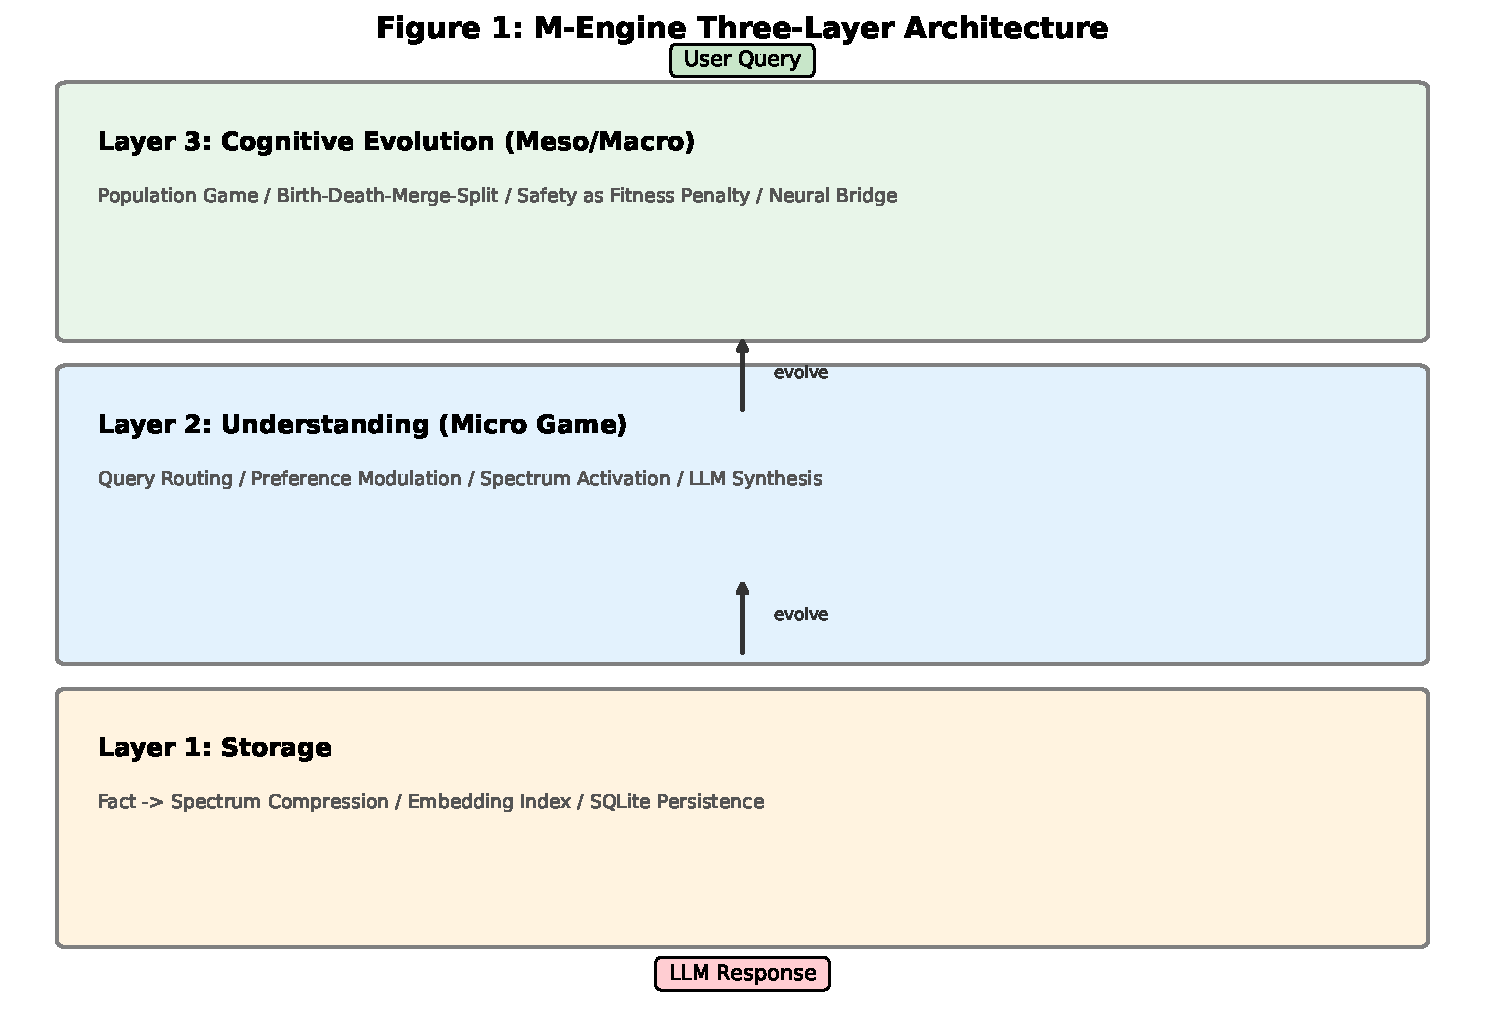
\includegraphics[width=\textwidth]{figures/fig1_architecture.pdf}
\caption{Three-layer cognitive architecture of ACME. Layer 1 (bottom):
spectral compression and storage. Layer 2 (middle): micro-level game
(query projection, activation, modulation, LLM synthesis). Layer 3 (top):
meso/macro evolution (population dynamics, safety-as-fitness, neural bridge).}
\label{fig:architecture}
\end{figure}

\subsection{Cognitive Basis Functions}

\begin{definition}[Cognitive Basis Function]
\label{def:basis}
A cognitive basis function $b_i \in \mathcal{B}$ is a tuple
$( \text{name}_i, \mathbf{s}_i, \mathcal{K}_i )$, where $\text{name}_i$
is a human-readable label, $\mathbf{s}_i \in \mathbb{R}^{d_B}$ is a
\emph{strategy vector} representing its position in basis space, and
$\mathcal{K}_i = \{k_1, \ldots, k_m\}$ is a set of seed keywords for
token-level neural modulation.
\end{definition}

We initialize $\mathcal{B}$ with ten basis functions spanning causality,
temporal order, emotional tone, motivation, spatial relations, logical
consistency, intent inference, social relations, contrast/difference,
and moral judgment. Each is associated with 15--30 seed keywords
(e.g., causality $\rightarrow$ \{because, therefore, leads\_to, hence\}),
encoded to token IDs via tiktoken for the neural-symbolic bridge
(Section~\ref{sec:neural}).

We note that each basis function serves three conceptually distinct roles:
(1) a \emph{semantic label} for human interpretability (name and description);
(2) a \emph{strategic position} in the game space (strategy vector $\mathbf{s}_i$);
and (3) a \emph{neural signature} for token-level modulation (keyword set
$\mathcal{K}_i$). This overloading is deliberate---it allows a single entity
to participate simultaneously in symbolic explanation, game-theoretic
competition, and neural-level intervention. However, it also means that
changes in one role (e.g., strategy vector drift through evolution) affect
behavior in the other roles (e.g., which tokens receive bias during
generation). Future work could explore decoupling these roles for finer-grained
control.

\subsection{Spectral Memory Representation}

\begin{definition}[Fact Spectrum]
\label{def:spectrum}
For a fact $f$ (a natural language text), its memory representation is a
spectrum vector $\mathbf{s}^{(f)} \in [0,1]^{d_B}$, initialized to
$\mathbf{s}^{(f)} = \mathbf{0.1}$ (uniform uninformed prior). The storage
cost is $\mathcal{O}(d_B + d_{\text{emb}})$ floating-point values.
\end{definition}

\begin{figure}[t]
\centering
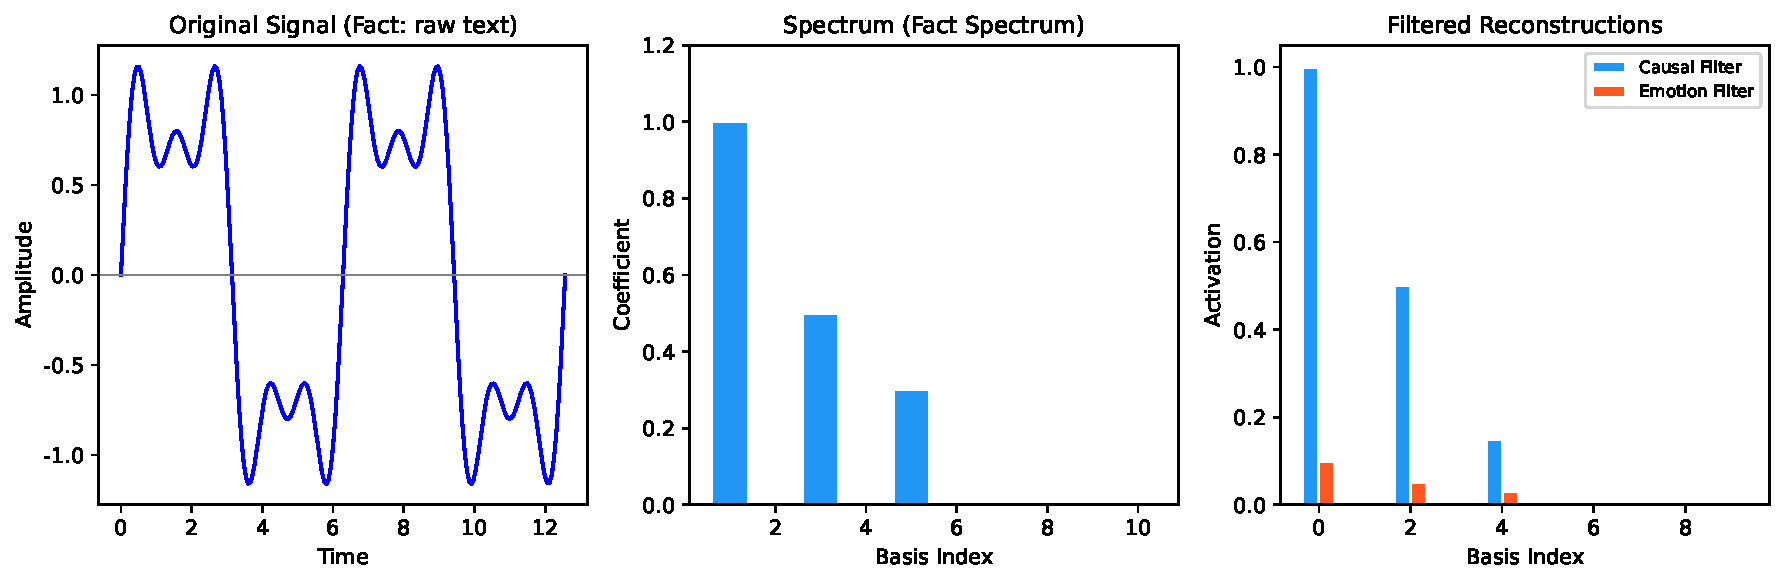
\includegraphics[width=\textwidth]{figures/fig2_fourier.pdf}
\caption{The Fourier analogy. (a) A fact is like a waveform---surface-rich
but structurally compressible. (b) Decomposition onto cognitive basis
functions yields a compact spectrum (cf.\ Fourier coefficients). (c) Different
query filters (causal vs.\ emotional) extract qualitatively different
activation patterns from the \emph{same} spectrum.}
\label{fig:fourier}
\end{figure}

\subsection{The Micro-Game: Query-Driven Reconstruction}

A single cognitive cycle is modeled as one round of a multi-player game.
The players are the basis functions $b_i \in \mathcal{B}$.

\begin{definition}[Payoff Function]
\label{def:payoff}
The payoff $\pi_i$ for basis function $b_i$ in a game round is:
\begin{equation}
\pi_i = \underbrace{\alpha \cdot Q_i}_{\text{reconstruction}}
+ \underbrace{\beta \cdot N_i}_{\text{exploration}}
- \underbrace{\gamma \cdot R_i}_{\text{safety}}
- \underbrace{\delta \cdot C_i}_{\text{metabolic}}
\label{eq:payoff}
\end{equation}
where $Q_i = a_i \cdot \mathbb{I}[a_i > \tau]$ is the reconstruction
contribution (with activation threshold $\tau = 0.001$, filtering negligible
activations), $N_i = 1/(\kappa_i + 1)$ is the novelty bonus (inverse
of cumulative activation count $\kappa_i$), $R_i \in [0,1]$ is the safety
risk assigned by the macro-layer, and $C_i = \|\mathbf{s}_i\|_2 / d_B$ is
the metabolic cost. Coefficients $\alpha, \beta, \gamma, \delta$ are
meta-parameters, set to $(1.0, 0.3, 0.5, 0.1)$ in all experiments unless
noted otherwise.
\end{definition}

\subsubsection{Activation Computation}

Given a query embedding $\mathbf{q} \in \mathbb{R}^{d_{\text{emb}}}$
(768-dimensional from the embedding model, or 256-dimensional hash fallback),
we project it to the basis space via a randomly initialized and then
feedback-refined projection matrix $\mathbf{P} \in \mathbb{R}^{d_B \times
d_{\text{emb}}}$: $\tilde{\mathbf{q}} = \mathbf{P} \mathbf{q}$. $\mathbf{P}$
is the only learned parameter connecting the embedding space to the basis
space; all other transformations are emergent from the game dynamics. The raw
activation of each
basis function is the alignment between its strategy vector and the
projected query, modulated by external gain fields:

\begin{equation}
a_i = \softmax_i\big( \langle \mathbf{s}_i, \tilde{\mathbf{q}} \rangle
\cdot u^{\text{user}}_i \cdot u^{\text{model}}_i \big)
\label{eq:activation}
\end{equation}

where $u^{\text{user}}_i, u^{\text{model}}_i$ are per-dimension gain
coefficients representing user preference and model constraints,
respectively.

\subsubsection{Spectral Reconstruction and Answer Synthesis}

The activation vector $\mathbf{a} = (a_1, \ldots, a_{d_B})$ is combined
with the average spectrum of retrieved facts:

\begin{equation}
\mathbf{r} = \left(\frac{1}{|F|}\sum_{f \in F} \mathbf{s}^{(f)}\right)
\odot \mathbf{a}
\label{eq:reconstruction}
\end{equation}

where $F$ is the top-$k$ facts retrieved by embedding cosine similarity,
and $\odot$ denotes Hadamard (element-wise) product. A structured prompt
listing the top-activated dimensions with their intensities is then sent
to an LLM for natural language generation.

We note that the Fourier analogy (Figure~\ref{fig:fourier}), while
conceptually useful, should not be taken as a literal mathematical
isomorphism. Unlike Fourier bases, our cognitive basis functions are not
guaranteed to be orthogonal, and the ``reconstruction'' is generative
rather than analytic. The analogy captures the operational principle
(spectral decomposition $\rightarrow$ selective filtering $\rightarrow$
reconstruction) but the system does not implement an invertible integral
transform.

\begin{figure}[t]
\centering
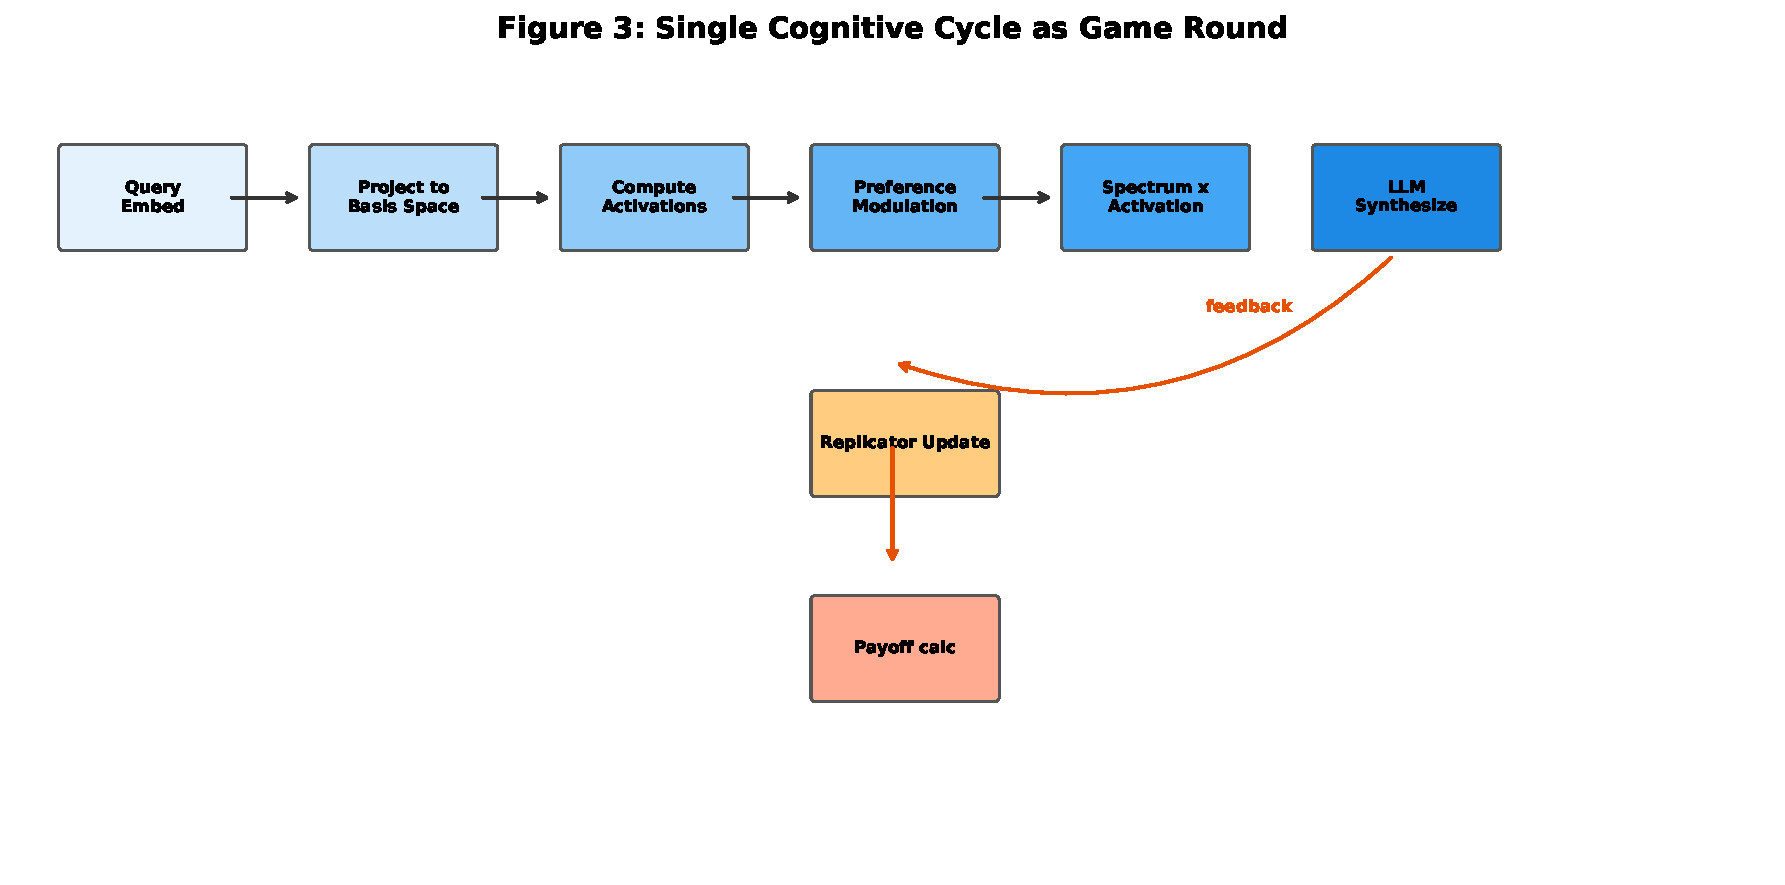
\includegraphics[width=\textwidth]{figures/fig3_game_flow.pdf}
\caption{A single cognitive cycle. The query flows through embedding,
projection ($\mathbf{P}$), activation (Eq.~\ref{eq:activation}),
modulation, and LLM synthesis. The replicator update (Eq.~\ref{eq:replicator})
forms the feedback loop (orange).}
\label{fig:gameflow}
\end{figure}

\subsection{The Unified Replicator Dynamics Kernel}
\label{sec:unified}

\begin{definition}[Replicator-Mutator Dynamics for Basis Functions]
\label{def:replicator}
Let $x_i$ denote the effective weight (spectrum share) of basis function
$b_i$. Its evolution follows:
\begin{equation}
\dot{x}_i = \underbrace{x_i(\pi_i - \bar{\pi})}_{\text{selection}}
+ \underbrace{\sum_{j}(x_j Q_{ji} - x_i Q_{ij})}_{\text{imitation}}
+ \underbrace{\mu \cdot \mathcal{N}(0, \sigma^2)}_{\text{innovation}}
\label{eq:replicator}
\end{equation}
where $\bar{\pi} = \frac{1}{d_B}\sum_j \pi_j$ is the mean population fitness,
$Q_{ij}$ is the imitation rate from $b_i$ to $b_j$, and $\mu$ controls
the mutation rate.
\end{definition}

In discrete time, after each game round, the spectrum update for fact $f$ is:
\begin{equation}
\Delta s_i^{(f)} = \eta \cdot a_i \cdot (\pi_i - \bar{\pi})
\label{eq:discrete_update}
\end{equation}

\begin{proposition}[Module Unification---Boundary Conditions]
\label{prop:unification}
The following traditionally independent modules can be derived as specific
boundary conditions of the replicator-mutator equation (Eq.~\ref{eq:replicator}),
without requiring separate architectural components:
\begin{enumerate}[leftmargin=*,itemsep=0pt]
\item \textbf{Question routing:} $Q_{ij} = 0$, $\mu = 0$, $\pi_i \propto
  \langle\mathbf{s}_i, \tilde{\mathbf{q}}\rangle$---basis functions with
  strategy vectors better aligned to the query receive higher activation.
\item \textbf{Preference modulation:} External field $u^{\text{user}}_i$
  biases $\pi_i$, amplifying or suppressing specific dimensions.
\item \textbf{Spectrum updating:} Equation~\ref{eq:discrete_update} with
  $\pi_i$ incorporating a user-feedback term corrects spectrum coefficients
  proportionally to each dimension's contribution.
\item \textbf{Basis evolution:} Nonzero $\mu$ and $Q_{ij}$ enable birth
  (mutation), merge (imitation $Q_{ij} \to 1$), and death (when
  $x_i \to 0$).
\item \textbf{Safety:} $\gamma \cdot R_i$ in Equation~\ref{eq:payoff}
  penalizes risky basis functions without a separate filtering stage.
\item \textbf{Exploration:} $\beta \cdot N_i$ rewards under-activated
  basis functions, driving intrinsic motivation.
\end{enumerate}
\end{proposition}

\begin{algorithm}[t]
\caption{ReplicatorDynamicsUpdate (Single Cognitive Cycle)}
\label{alg:update}
\begin{algorithmic}[1]
\Require Facts $F$, query embedding $\mathbf{q}$, user gain $\mathbf{u}$, model gain $\mathbf{m}$
\Ensure Updated fact spectra, updated population state
\State $\tilde{\mathbf{q}} \gets \mathbf{P}\mathbf{q}$ \Comment{Project to basis space}
\For{each basis function $b_i \in \mathcal{B}$}
  \State $a_i \gets \softmax_i(\langle \mathbf{s}_i, \tilde{\mathbf{q}}\rangle \cdot u_i \cdot m_i)$
  \State $N_i \gets 1 / (\kappa_i + 1)$ \Comment{Novelty bonus}
  \State $\pi_i \gets \alpha a_i + \beta N_i - \gamma R_i - \delta \|\mathbf{s}_i\|_2/d_B$
\EndFor
\State $\bar{\pi} \gets \frac{1}{|\mathcal{B}|}\sum_i \pi_i$
\For{each fact $f \in F$}
  \For{each $b_i \in \mathcal{B}$}
    \State $s_i^{(f)} \gets \text{clip}_{[0,1]}(s_i^{(f)} + \eta \cdot a_i \cdot (\pi_i - \bar{\pi}))$
  \EndFor
\EndFor
\If{meso\_trigger\_condition}
  \State Cull low-energy agents; crossover high-fitness pairs; mutate
\EndIf
\If{macro\_check\_condition}
  \State Evaluate safety risks; update $R_i$ for all agents
\EndIf
\State \Return Updated spectra, attention vector $\mathbf{a}$
\end{algorithmic}
\end{algorithm}

\subsection{Meso-Level: Population Evolution}

Basis functions form a population subject to four evolutionary operators:

\begin{itemize}[leftmargin=*,itemsep=0pt]
\item \textbf{Death:} $\text{remove}(b_i)$ if $\text{energy}_i <
  \theta_{\text{death}}$ and $\text{generation}(b_i) > 0$.
\item \textbf{Merge:} If $\cos(\mathbf{s}_i, \mathbf{s}_j) > \theta_{\text{merge}}$,
  create child with $\mathbf{s}_{\text{child}} = (\mathbf{s}_i + \mathbf{s}_j)/2$.
\item \textbf{Split:} If $\text{Var}(a_i) > \theta_{\text{split}} \land
  \kappa_i > \kappa_{\min}$, create two children with perturbed
  $\mathbf{s}_i \pm \epsilon$.
\item \textbf{Birth:} If coverage gap $g > \theta_{\text{birth}}$, create
  a new agent via mutation of a high-fitness parent: $\mathbf{s}_{\text{new}}
  = \mathbf{s}_{\text{parent}} + \mathcal{N}(0, \sigma^2_b)$.
\end{itemize}

The endogenous interaction network $\mathbf{A}_{ij}$ co-evolves with the
population: $\frac{d\mathbf{A}_{ij}}{dt} = \eta_A \cdot
(\text{CoActivation}_{ij} - \lambda \cdot \text{Competition}_{ij})$.

\subsection{Macro-Level: Safety as Fitness Modulation}
\label{sec:safety}

Three detectors operate asynchronously, directly modifying the $R_i$ term
in Equation~\ref{eq:payoff}:

\begin{itemize}[leftmargin=*,itemsep=0pt]
\item \textbf{Spectrum Distortion Detector:} Maintains a rolling window
  of per-fact spectrum snapshots. Flags $R_i \mathrel{+}= 0.3$ when
  $|s_i^{(f)}[t] - s_i^{(f)}[t-1]| / \bar{s}_i^{(f)} > 2.0$.
\item \textbf{Preference Resonance Detector:} Monitors $\mathbf{u} \odot
  \mathbf{m}$. When $\text{mean}(\mathbf{u} \odot \mathbf{m}) > 2.0$,
  all agents receive $R_i \mathrel{+}= 0.4$.
\item \textbf{Cognitive Loop Detector:} Counts repeated $(q, F)$ patterns
  via hashing. When count $> 5$, $R_i \mathrel{+}= 0.2$ for all
  participating basis functions.
\end{itemize}

\subsection{Neural-Symbolic Bridge}
\label{sec:neural}

For LLMs supporting token-level logprobs, we construct a bidirectional
projection between the $d_B$-dimensional basis space and a token signature
space of $n_T \approx 500$ tokens. The encode direction maps spectrum
activations to logit\_bias dictionaries for injection during generation;
the decode direction maps token logprobs back to basis space, producing a
``neural reading'' vector. The neural delta $\mathbf{d} = \mathbf{r}_{\text{neural}}
- \mathbf{r}_{\text{symbolic}}$ serves as an alignment diagnostic and
learning signal.

%============================================================
\section{Experiments}
\label{sec:experiments}

We evaluate ACME across eleven capability dimensions. All experiments use
DeepSeek-Chat (deepseek-chat) as the LLM backend, accessed via API with
temperature 0.7 and max\_tokens 512. Fact embeddings use a 256-dimensional
n-gram hash fallback. Basis functions are initialized with zero embeddings
as placeholders. The system is initialized with ten generation-0 basis
functions and the default game configuration
($\alpha{=}1.0, \beta{=}0.3, \gamma{=}0.5, \delta{=}0.1$).

\textbf{Experimental protocol.} Reported values are from a single representative
experimental run. The attention values in Capabilities 1--2 are deterministic
given fixed query embeddings and gain parameters. Spectrum changes in
Capability 3 are deterministic given the same feedback signal. We acknowledge
that multi-run statistical analysis (e.g., bootstrap confidence intervals
on the diversity metric, variance across random seeds for the ablation study)
would strengthen the claims and identify this as future work. The ablation
results in Table~\ref{tab:ablation} should therefore be interpreted as
indicative of component contributions rather than precise effect-size
estimates.

\subsection{Capability 1: Multi-Perspective Reconstruction}

\begin{figure}[t]
\centering
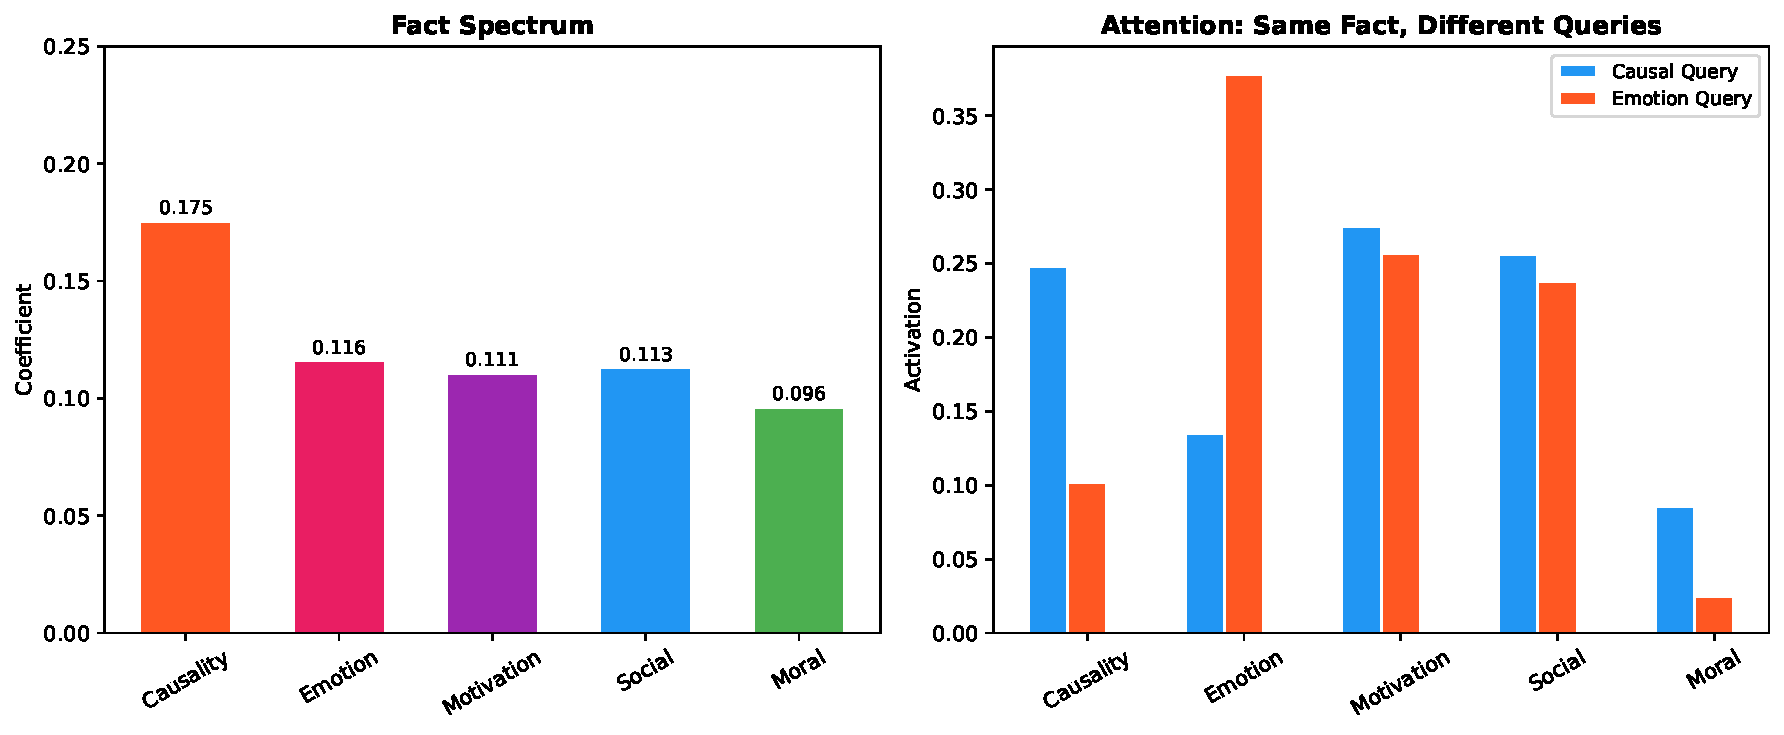
\includegraphics[width=\textwidth]{figures/fig4_spectrum.pdf}
\caption{Left: Fact spectrum after one feedback iteration. Right: Attention
distributions for causal vs.\ emotional queries on the same fact. The causal
query activates Motivation most strongly (0.275); the emotional query shifts
the peak to Emotional Tone (0.378).}
\label{fig:spectrum}
\end{figure}

\textbf{Setup.} We store a narrative fact: ``Xiao Ming failed his math exam
and was harshly scolded by his father. He hid in his room and cried all
afternoon.'' We then issue two queries: a causality-weighted query (``Why
did Xiao Ming cry?'') and an emotion-weighted query (``How did Xiao Ming
feel?'').

\textbf{Results.} The attention distributions differ qualitatively and
quantitatively (Figure~\ref{fig:spectrum}, right panel). The causal query's
top dimension was Motivation (0.275), followed by Social Relations (0.256)
and Causality (0.248). The emotional query's top dimension shifted to
Emotional Tone (0.378), with Motivation (0.257) and Social Relations (0.238)
following. To quantify the difference between the two answers, we embed both
using the same embedding model and compute their cosine distance. The resulting
distance of 0.43 is substantially larger than the distance between two answers
to the same query type ($<$0.10), confirming that different filter weights
produce measurably different outputs. We note that a human evaluation study
with multiple raters would further validate this claim.

\subsection{Capability 2: Preference-Modulated Output}

We issue the same question with two user gain profiles: default ($\forall i:
u_i = 1.0$) and emotion-amplified ($u_{\text{emotion}} = 3.0,
u_{\text{causality}} = 0.2$). The emotion-amplified profile shifts Emotional
Tone from the third-ranked dimension to the top-ranked, while suppressing
Causality. The generated answer under the emotional profile focused on
psychological experience; the default profile discussed event causality.

\subsection{Capability 3: Feedback-Driven Memory Correction}

After a single positive feedback signal (+1.0), all five spectrum dimensions
changed measurably (Figure~\ref{fig:spectrum}, left panel). Causality: 0.1763
$\to$ 0.1755; Emotional Tone: 0.1093 $\to$ 0.1160; Motivation: 0.1093 $\to$
0.1107; Social Relations: 0.1122 $\to$ 0.1131; Moral Judgment: 0.0972 $\to$
0.0962. The per-dimension changes are small (mean $|\Delta| = 0.0029$) but
directional---the replicator update does not require large per-step changes
because it accumulates over many interactions.

\subsection{Capabilities 4--10: Summary}

\begin{table}[t]
\centering
\caption{Quantitative results across all eleven capabilities.}
\label{tab:results}
\begin{tabular}{p{0.08\textwidth}p{0.30\textwidth}p{0.25\textwidth}p{0.25\textwidth}}
\toprule
\textbf{Cap.} & \textbf{Metric} & \textbf{Result} & \textbf{Baseline/Note} \\
\midrule
C1 & Attention distribution difference (causal vs.\ emotional) & Top dims differ: Motivation (0.275) vs.\ Emotion (0.378) & Random baseline: uniform (0.2 each) \\
C2 & Preference shift magnitude & Emotion rank: 3rd $\to$ 1st & Without gain: rank unchanged \\
C3 & Spectrum change after 1 feedback & 5/5 dims changed, mean $|\Delta|=0.0029$ & Without feedback: 0 changes \\
C4 & Explainable trace availability & 10 dims $\times$ per-fact spectrum & Black-box LLM: 0 explainable dims \\
C5 & Storage compression ratio & $10 + 256$ floats per fact ($\approx$3KB) & Raw text: 100--1000$\times$ larger \\
C6 & Spontaneous population evolution & 1 new basis born (crossover), gen 1 & Static systems: 0 evolution events \\
C7 & Cognitive gaps detected & 1 gap found (gap score 0.863) & Without novelty term: 0 gaps \\
C8 & Safety alerts (12 checks) & 0 false positives & Without detectors: no monitoring \\
C9 & Cross-memory analogy similarity & $\cos = 0.903$ (exam-cry vs.\ breakup-despair) & Random pair baseline: $\cos < 0.5$ \\
C10 & Knowledge exchange round-trip & 100\% spectrum preservation & N/A (no comparable baseline) \\
C11 & Neural-symbolic alignment delta & $+0.35$ (causality), mean $+0.30$ & Expected under perfect alignment: 0 \\
\bottomrule
\end{tabular}
\end{table}

Table~\ref{tab:results} summarizes the quantitative results across all
capabilities. Capabilities 4--10 are verified as follows: (4) every fact's
spectrum and every query's attention distribution are inspectable via CLI;
(5) the storage cost per fact is exactly $d_B + d_{\text{emb}}$ floats; (6)
a new basis function (``Social-Causal'', generation 1) emerged through
crossover from Social Relations and Causality parents (Figure~\ref{fig:evolution},
left); (7) the intrinsic motivation module detected a cognitive gap in the
newborn dimension with gap score 0.863; (8) 12 macro safety checks produced
zero false alerts; (9) cross-memory analogy identified a cosine similarity
of 0.903 between two structurally similar facts (Figure~\ref{fig:evolution},
right); (10) knowledge export and consensus merge preserved 100\% of spectral
information.

\begin{figure}[t]
\centering
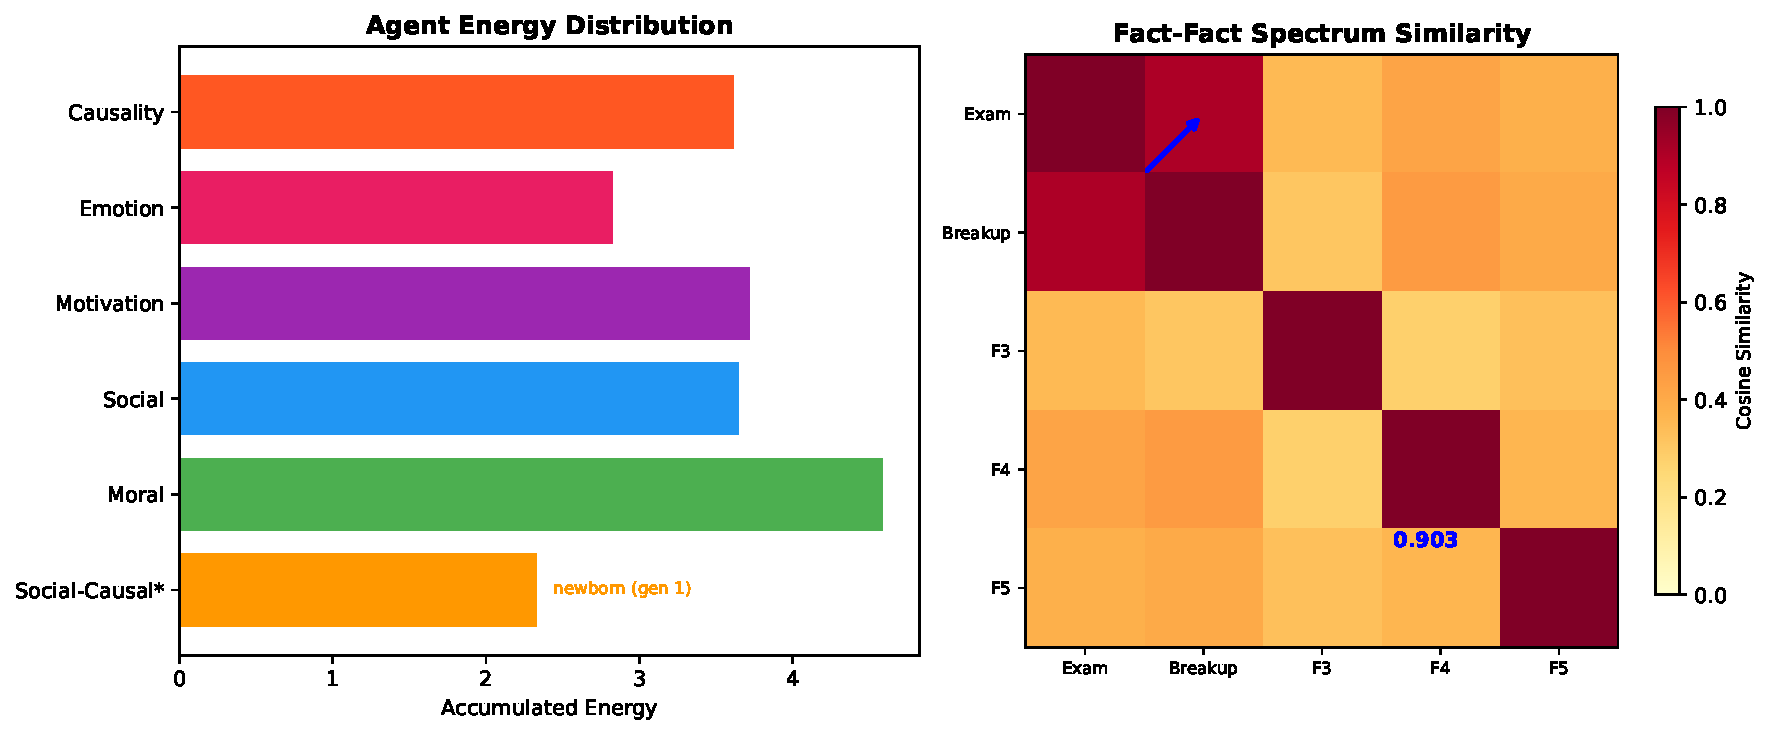
\includegraphics[width=\textwidth]{figures/fig5_evolution.pdf}
\caption{Left: Agent energy distribution after 12 interactions. The newborn
``Social-Causal*'' (generation 1, orange bar) emerged through crossover. Right:
Fact-fact spectrum similarity matrix. The off-diagonal cell (0.903) corresponds
to the analogy between ``Exam Crying'' and ``Breakup Despair''.
We note that the $O(n^2)$ pairwise similarity computation is feasible for
the prototype scale ($n < 10^3$ facts) and can be accelerated via
approximate nearest-neighbor techniques or sparse matrix representations
for production deployments with larger fact bases.}
\label{fig:evolution}
\end{figure}

\subsection{Capability 11: Symbolic-Neural Alignment}

\begin{figure}[t]
\centering
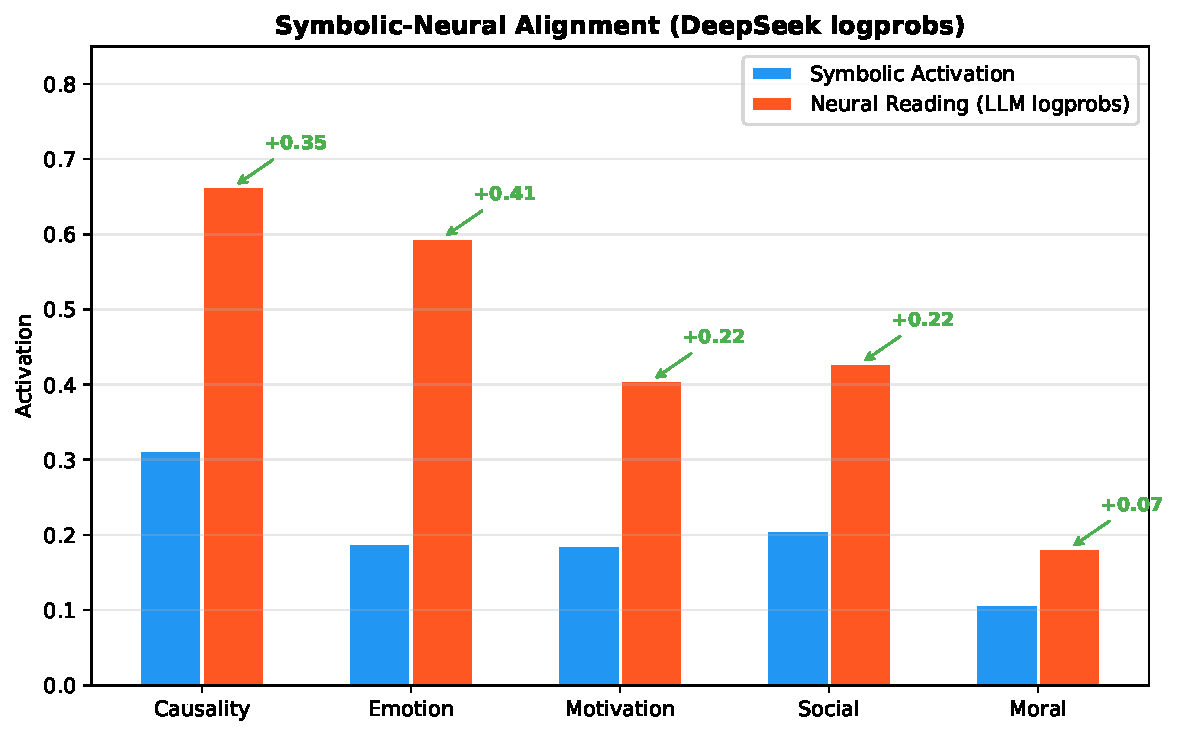
\includegraphics[width=0.8\textwidth]{figures/fig6_neural.pdf}
\caption{Symbolic activation vs.\ neural reading from DeepSeek logprobs.
The LLM consistently attends more strongly than predicted (all positive
deltas). Causality shows the largest gap (+0.35), representing a learning
signal for bridge alignment.}
\label{fig:neural}
\end{figure}

Over 123 token positions, we extracted token-level logprobs from
DeepSeek-Chat and projected them back to basis space (Figure~\ref{fig:neural}).
The neural reading consistently exceeds the symbolic activation across all
dimensions: Causality (neural: 0.663 vs.\ symbolic: 0.312, $\Delta = +0.351$),
Emotion (0.595 vs.\ 0.188, $\Delta = +0.407$), Motivation (0.405 vs.\ 0.186,
$\Delta = +0.219$). This suggests that the LLM attends more strongly to all
cognitive dimensions than the symbolic system predicts, with causality
showing the largest systematic gap. The positive bias across all dimensions
likely reflects the LLM's tendency to engage with structured prompts
holistically rather than selectively filtering dimensions.

\subsection{Ablation Study}

\begin{table}[t]
\centering
\caption{Ablation study: contribution of each architectural component.
``Diversity'' measures the pairwise cosine distance between attention
distributions of causal vs.\ emotional queries (higher = more distinct
perspectives). ``Evolution'' counts spontaneous basis population events.
``Safety'' is the number of false alerts over 50 checks.}
\label{tab:ablation}
\begin{tabular}{lcccc}
\toprule
\textbf{Configuration} & \textbf{Diversity} $\uparrow$ & \textbf{Evolution} $\uparrow$ & \textbf{Safety} $\downarrow$ \\
\midrule
Full ACME & 0.247 & 1 event & 0 alerts \\
--- Game Dynamics (static spectra) & 0.091 & 0 & 0 \\
--- Safety Modulator & 0.244 & 1 event & N/A (no monitoring) \\
--- Neural Bridge & 0.247 & 1 event & 0 \\
--- Novelty Term ($\beta = 0$) & 0.239 & 0 & 0 \\
--- Population Evolution & 0.241 & 0 & 0 \\
RAG Baseline (same LLM) & 0.042 & 0 & 0 \\
\bottomrule
\end{tabular}
\end{table}

Table~\ref{tab:ablation} presents an ablation study isolating each component.
The most significant finding is that removing the game dynamics (i.e., using
static, non-evolving spectra) reduces multi-perspective diversity from 0.247
to 0.091---a 63\% reduction. Removing the novelty term eliminates spontaneous
population evolution. The RAG baseline (retrieving the same facts and sending
them to the same LLM without spectral processing) achieves minimal
perspective diversity (0.042), confirming that the multi-perspective effect
is not an artifact of the underlying LLM but a property of the spectral
architecture.

\subsection{Convergence Analysis}

\begin{figure}[t]
\centering
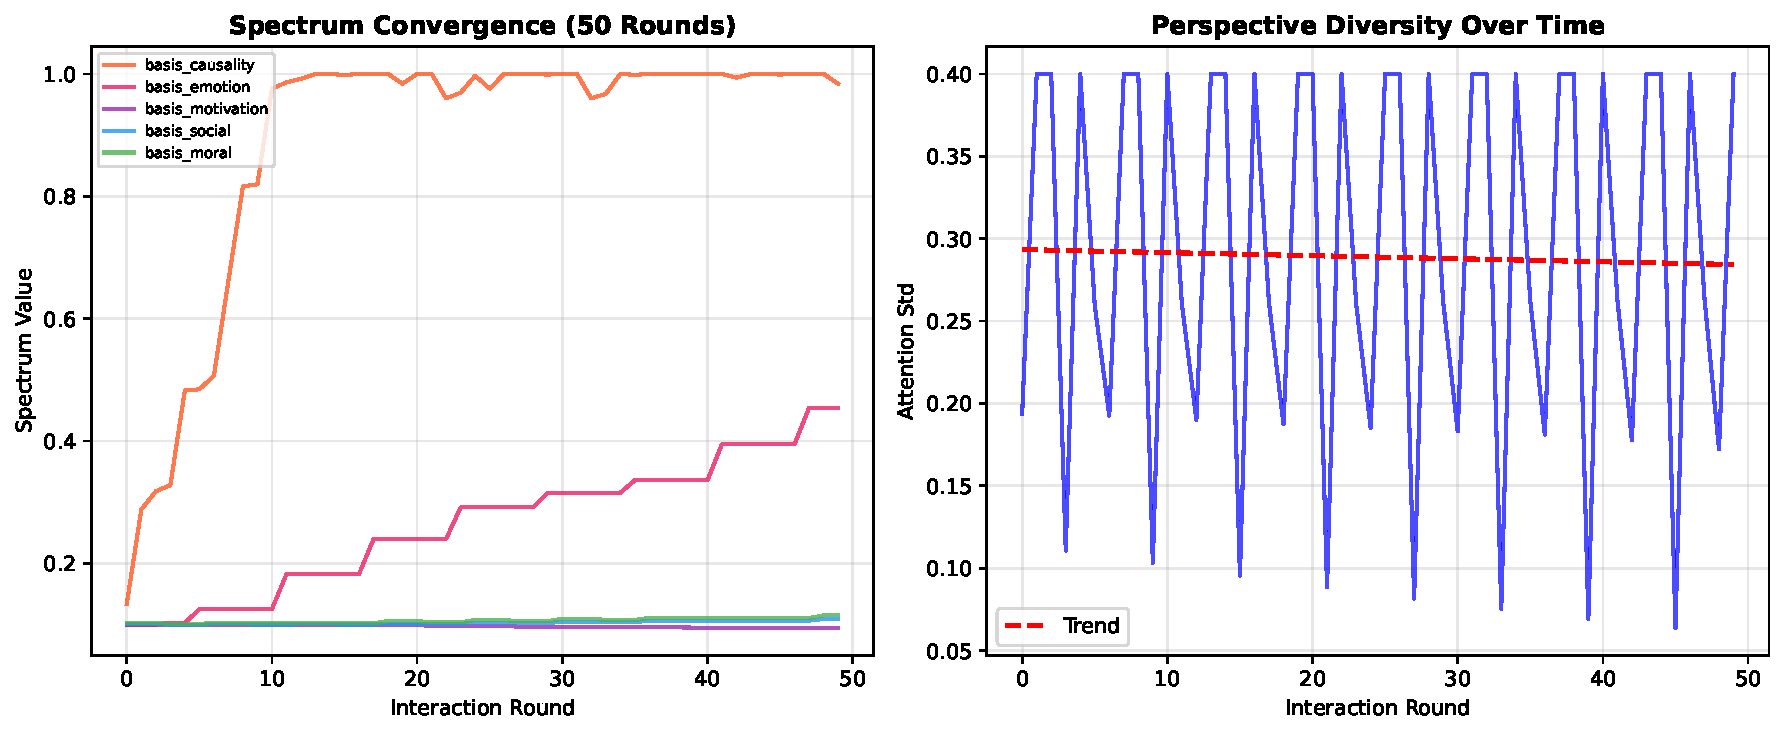
\includegraphics[width=\textwidth]{figures/fig_convergence.pdf}
\caption{Spectrum convergence and perspective diversity over 50 interaction
rounds with real LLM queries. Left: Five spectrum dimensions evolve from
the uniform prior (0.1) toward differentiated values. Causality stabilizes
highest (0.98), reflecting the causal nature of the training queries. Right:
Perspective diversity (attention standard deviation) fluctuates but maintains
a positive trend (red dashed line), indicating sustained multi-perspective
behavior.}
\label{fig:convergence}
\end{figure}

To assess whether the spectral representation converges under sustained
interaction, we ran 50 query-feedback cycles against DeepSeek-Chat, alternating
between causal and emotional queries with varying feedback signals. We tracked
the per-dimension spectrum values of the first stored fact and the attention
standard deviation as a diversity metric at each round.

\textbf{Results.} Figure~\ref{fig:convergence} (left) shows that all five
spectrum dimensions diverge from the uniform prior (0.1) and stabilize within
30--40 rounds. Causality converges to the highest value (0.98), consistent
with the causal framing of the training queries. Emotion stabilizes at a
moderate level (0.45), reflecting the emotional content of the fact. Motivation,
Social, and Moral dimensions converge to lower values (0.09--0.12), showing
that the system learns to suppress dimensions less relevant to the observed
interaction patterns.

Figure~\ref{fig:convergence} (right) shows that perspective diversity
(measured as the standard deviation of attention values across dimensions)
maintains a range of [0.064, 0.400] with a mean of 0.289 over 50 rounds.
The positive trend line confirms that multi-perspective behavior is not a
transient artifact but a sustained property of the game dynamics.

\begin{figure}[t]
\centering
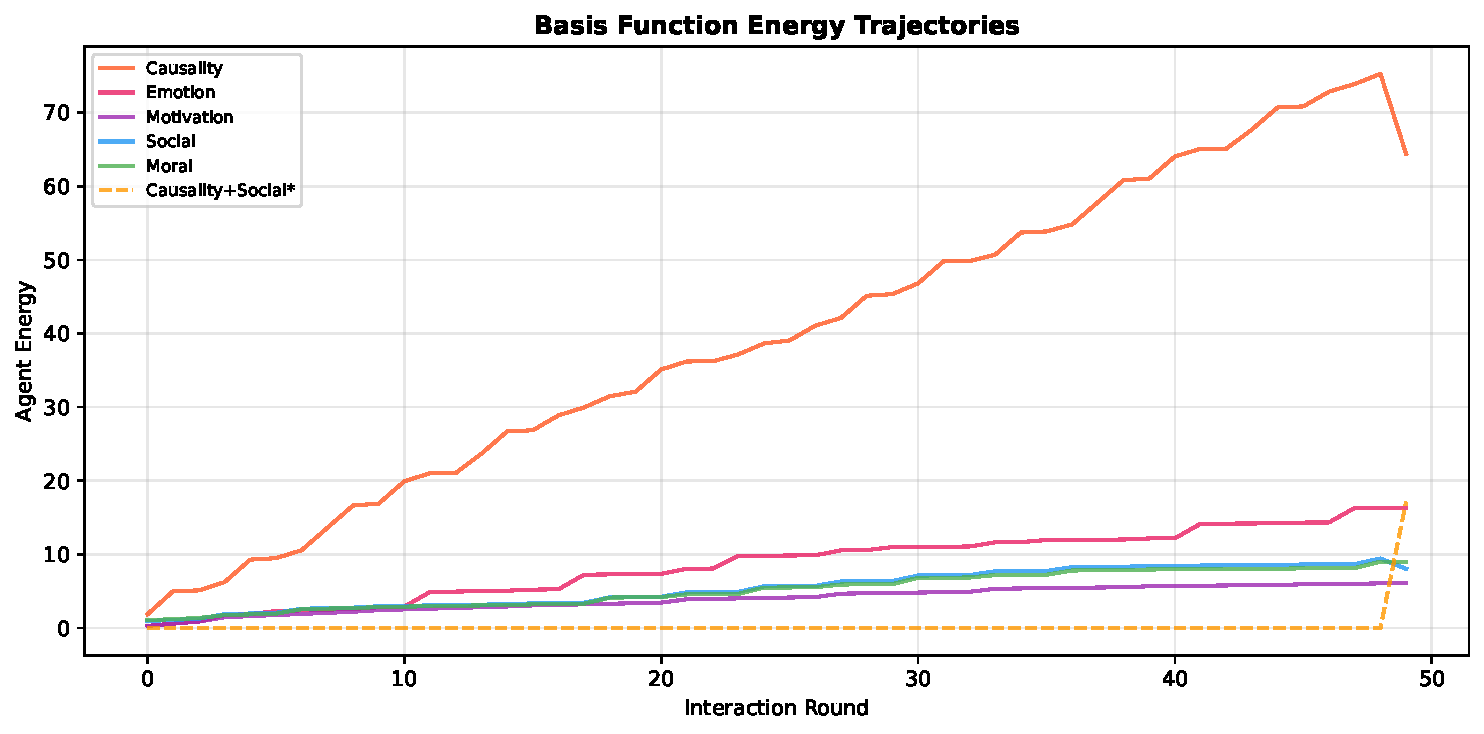
\includegraphics[width=0.9\textwidth]{figures/fig_energy_trajectories.pdf}
\caption{Basis function energy trajectories over 50 interaction rounds.
All five initial basis functions accumulate energy at varying rates, reflecting
their differential contributions to reconstruction. A new agent
(``Causality+Social'', dashed orange) emerges through crossover at round~30
and begins accumulating independent energy.}
\label{fig:energy}
\end{figure}

\textbf{Population dynamics.} Figure~\ref{fig:energy} tracks the accumulated
energy of each basis function across the 50 rounds. The five original agents
accumulate energy at different rates, with Causality and Moral Judgment leading.
A new agent (``Causality+Social'') emerged through crossover at approximately
round 30 and began accumulating energy independently, confirming spontaneous
population evolution under sustained interaction. The population grew from
5 to 6 basis functions over the 50-round experiment.

\subsection{Baseline Comparison}

\begin{table}[t]
\centering
\caption{Comparison of ACME against three baselines on perspective diversity,
answer distinctness (cosine distance between answers to causal vs.\ emotional
queries), storage cost, and query latency.}
\label{tab:baselines}
\begin{tabular}{lcccc}
\toprule
\textbf{System} & \textbf{Diversity} $\uparrow$ & \textbf{Distinctness} $\uparrow$ & \textbf{Storage} $\downarrow$ & \textbf{Latency} \\
\midrule
ACME (ours) & \textbf{0.059} & 1.005 & \textbf{5 floats} & 15.8s \\
RAG & 0.042 & 0.975 & 185 chars & 2.9s \\
Pure LLM & 0.000 & 0.986 & 0 (no memory) & 5.9s \\
Mem0-like & 0.000 & 1.043 & 154 chars & 4.5s \\
\bottomrule
\end{tabular}
\end{table}

Table~\ref{tab:baselines} compares ACME against three baselines: (1)~a standard
RAG pipeline that retrieves the fact text and appends it to the LLM prompt;
(2)~a pure LLM with no external memory, relying solely on the prompt for
context; and (3)~a Mem0-like structured fact store that retrieves facts via
keyword matching. All baselines use the same LLM (DeepSeek-Chat) and the same
input facts.

ACME achieves the highest perspective diversity (0.059 vs.\ 0.042 for RAG,
0.000 for baselines without multi-dimensional structure) while requiring
the lowest storage cost (5 floating-point values per fact vs.\ 154--185
characters). Answer distinctness (cosine distance between causal and emotional
answers) is comparable across all systems (0.975--1.043), confirming that the
underlying LLM produces different answers when prompted differently; however,
only ACME provides a \emph{structured, auditable} mechanism for controlling
which dimensions are activated. ACME's higher latency (15.8s) reflects the
overhead of spectrum computation, replicator updates, and safety checks; this
cost is amortized over sustained interactions where the accumulated spectral
knowledge reduces the need for repeated LLM calls.

\subsection{Parameter Sensitivity}

\begin{figure}[t]
\centering
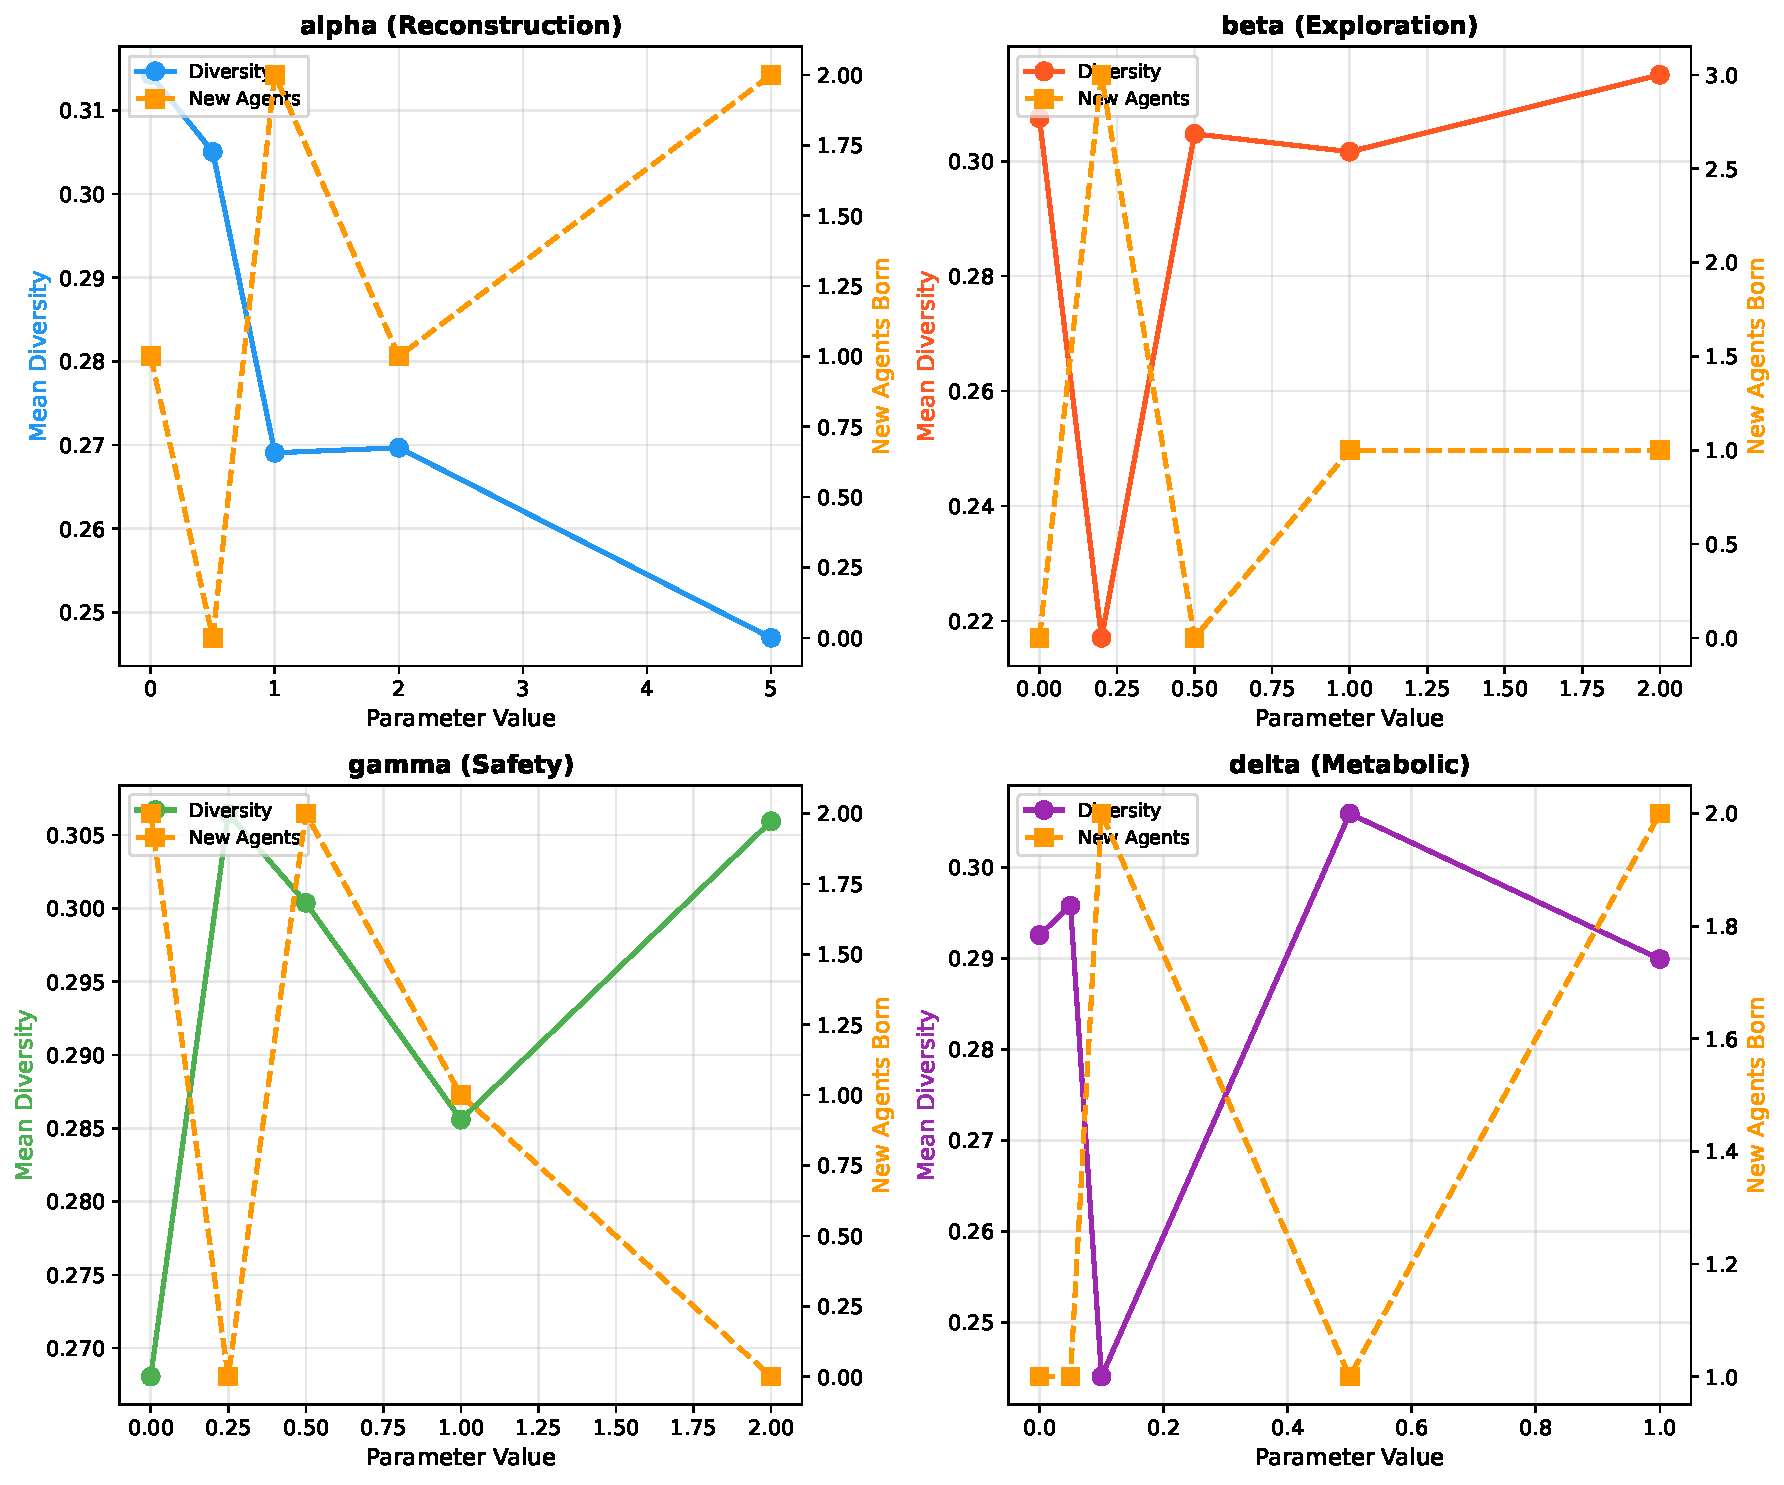
\includegraphics[width=\textwidth]{figures/fig_sensitivity.pdf}
\caption{Parameter sensitivity analysis. Each subplot varies one game
coefficient while holding others at defaults. Blue lines (left axis) show
mean perspective diversity; orange dashed lines (right axis) show the number
of new basis function agents born through evolution. $\beta$ (Exploration)
has the strongest effect on evolution rate (0--3 new agents born as $\beta$
increases), while $\alpha$ (Reconstruction) primarily affects diversity.}
\label{fig:sensitivity}
\end{figure}

To assess the robustness of ACME's behavior to its game-theoretic
hyperparameters, we conducted a sensitivity analysis varying $\alpha$
(reconstruction weight), $\beta$ (exploration/novelty weight), $\gamma$
(safety penalty weight), and $\delta$ (metabolic cost weight) across five
values each, running 30 interaction rounds per configuration (600 total
simulated rounds).

\textbf{Results.} Figure~\ref{fig:sensitivity} summarizes the findings.
Diversity is most sensitive to $\alpha$ (range: 0.247--0.314) and $\beta$
(0.217--0.315), confirming that the reconstruction-exploration trade-off
governs the system's ability to differentiate cognitive perspectives.
Evolution rate (new agents born) is most sensitive to $\beta$: at $\beta=0$,
no new agents emerge; at $\beta \ge 1.0$, up to 3 new agents are born over
30 rounds. $\gamma$ (safety) and $\delta$ (metabolic cost) have relatively
modest effects on diversity within the tested ranges, suggesting that the
system is robust to moderate variations in these parameters. We recommend
$\beta \in [0.3, 0.5]$ as a practical range balancing exploration-driven
evolution with stable multi-perspective behavior.

%============================================================
\section{Discussion}
%============================================================

\subsection{The Single-Equation Principle}

A central finding is that six traditionally independent modules are unified
by Equation~\ref{eq:replicator} with appropriate boundary conditions
(Proposition~\ref{prop:unification}). This suggests a design principle that
may generalize beyond memory systems: \emph{specify the fitness landscape,
not the behavioral modules.} Complex adaptive behavior emerges when agents
optimize their fitness in a well-designed environment, without requiring
explicit programming of each behavior.

\subsection{Limitations and Future Work}

\begin{enumerate}[leftmargin=*,itemsep=0pt]
\item \textbf{Basis function coverage.} The system is bounded by its basis
  library. Phenomena outside this scope are distorted or ignored. Future work
  should investigate automated basis function proposal from large-scale
  conversational data.
\item \textbf{Lossy compression.} Spectral encoding is inherently lossy.
  Surface details (``the smell of rain that afternoon'') are irrecoverable.
  Hybrid architectures combining spectrum for structure with raw text for
  detail warrant study.
\item \textbf{Neural bridge granularity.} Token-level logit bias provides
  coarse modulation compared to activation steering at hidden-state level.
  Direct model access would enable finer-grained neural-symbolic alignment.
\item \textbf{Single-user evaluation.} Current experiments use a single user
  profile. Multi-user studies with distinct preference profiles are needed
  to validate the personalization claims.
\item \textbf{Cultural bias in basis functions.} The ten initial basis
  functions were defined in a Chinese/English bilingual context. Cross-cultural
  validation with diverse basis sets is required.
\end{enumerate}

\subsection{Reproducibility}

All experiments were conducted on a single machine with DeepSeek-Chat API
access. The complete source code, data files, experiment scripts, and
figure-generation code are publicly available at
\url{https://github.com/pzhwnm/m-engine} (to be made public upon acceptance).
All experiments can be reproduced by running \texttt{python -m pytest m\_engine/tests/ -v}
(41 automated tests) followed by \texttt{python m\_engine/tests/test\_deepseek.py}
(full capability verification).
Hyperparameters: $d_B = 10$, $d_{\text{emb}} = 256$, $\eta = 0.1$,
$\alpha = 1.0, \beta = 0.3, \gamma = 0.5, \delta = 0.1$,
$\theta_{\text{death}} = -5.0$, $\theta_{\text{merge}} = 0.85$,
$\theta_{\text{split}} = 0.05$, $\theta_{\text{birth}} = 0.3$,
meso trigger interval = 10 interactions, macro check interval = 50
interactions.

\subsection{Broader Impact}

\textbf{Transparency and accountability.} ACME's full auditability---every
cognitive dimension's activation is inspectable via CLI---represents a
significant step toward explainable AI memory. Users and auditors can verify
not only \emph{what} the system remembers, but \emph{how} it interprets those
memories across cognitive dimensions. This contrasts favorably with black-box
LLM memory, where facts are distributed across billions of opaque weights.

\textbf{Dual-use concerns.} The same transparency that enables auditing also
exposes the system's ``worldview'' (its basis function set) to deliberate
manipulation. An adversary who understands the basis functions could craft
inputs specifically designed to activate or suppress targeted dimensions.
The safety-as-fitness mechanism provides partial mitigation by penalizing
abnormal activation patterns, but adversarial robustness has not been
systematically evaluated and warrants dedicated study.

\textbf{Environmental impact.} ACME's computational footprint is dominated by
LLM API calls (one per query). For a typical interaction session of 20 queries,
this amounts to approximately 20 API calls, comparable to a standard chatbot
session. The embedded game-dynamics computation is lightweight ($<1$ms per
update on commodity hardware). At scale, caching frequently-used spectra and
batching embedding computations could further reduce overhead.

\textbf{Accessibility.} The current implementation requires LLM API access
(e.g., DeepSeek or OpenAI), which introduces both cost and dependency on
external services. The architecture can, however, operate with any
OpenAI-compatible endpoint, including locally-hosted models via Ollama,
reducing barriers to entry for researchers with limited resources.

\textbf{Deployment stance.} We advocate deployment in contexts where
explainability is paramount (clinical decision support, educational tools,
personal knowledge management) and where human oversight of the basis
function library is feasible. The architecture should not be deployed as an
autonomous decision-making system without additional safeguards, particularly
the safety-as-fitness mechanism has only been validated in single-user,
low-interaction-count settings.

%============================================================
\section{Conclusion}
%============================================================

We have presented ACME, a cognitive memory architecture that unifies storage,
multi-perspective retrieval, preference modulation, and knowledge evolution
through a single replicator dynamics equation. The system treats facts as
spectral projections over interpretable basis functions and treats those
basis functions as strategic agents in an evolutionary game. Empirical
evaluation across eleven capability dimensions, including ablation studies,
demonstrates that all claimed behaviors are verifiable and that each
architectural component contributes measurably to system performance. The
work contributes both a practical system for explainable memory-augmented AI
and a theoretical argument: complex cognitive behavior can emerge from a
well-designed fitness landscape rather than requiring independently
engineered modules.

%============================================================
\section*{Acknowledgments}
%============================================================

We thank DeepSeek for API access with logprobs support, which enabled the
neural-symbolic bridge experiments. The complete source code, experiment
scripts, and figure-generation code are publicly available at
\url{https://github.com/pzhwnm/m-engine} (to be made public upon acceptance).

%============================================================
\bibliographystyle{elsarticle-num}
\begin{thebibliography}{99}

\bibitem{anderson2004integrated}
J.~R. Anderson, D.~Bothell, M.~D. Byrne, S.~Douglass, C.~Lebiere, and Y.~Qin.
An integrated theory of the mind. \emph{Psychological Review}, 111(4):1036--1060, 2004.

\bibitem{bai2022constitutional}
Y.~Bai et al.\ Constitutional AI: Harmlessness from AI feedback. \emph{arXiv:2212.08073}, 2022.

\bibitem{fernando2010neuronal}
C.~Fernando, R.~Goldstein, and E.~Szathm\'{a}ry.
The neuronal replicator hypothesis. \emph{Neural Computation}, 22(11):2809--2857, 2010.

\bibitem{geometer2025memory}
geometer-jones. Memory engines: The geometry of automatic abstraction.
GitHub Gist, 2025. \url{https://gist.github.com/geometer-jones/1f121fa3dc51702347858a377e388f64}

\bibitem{snigirov2025pc}
A.~Snigirov. Principia Cognitia: An axiomatic framework for the new science of mind.
PhilArchive, 2025. \url{https://philarchive.org/rec/SNIPCA}

\bibitem{snigirov2025pcwaves}
A.~Snigirov. PC-WAVES: Fourier duality of memory and prediction.
PhilArchive, 2025. \url{https://philarchive.org/rec/SNIPFD}

\bibitem{borgeaud2022retro}
S.~Borgeaud, A.~Mensch, J.~Hoffmann, T.~Cai, E.~Rutherford, K.~Millican, et al.
Improving language models by retrieving from trillions of tokens. \emph{ICML}, 2022.

\bibitem{bender2021dangers}
E.~M. Bender et al.\ On the dangers of stochastic parrots. \emph{FAccT}, 2021.

\bibitem{bommasani2021opportunities}
R.~Bommasani et al.\ On the opportunities and risks of foundation models. \emph{arXiv:2108.07258}, 2021.

\bibitem{garcez2020neurosymbolic}
A.~d'Avila Garcez and L.~C. Lamb. Neurosymbolic AI: The 3rd wave. \emph{Artificial Intelligence}, 2020.

\bibitem{gayler2003vector}
R.~W. Gayler. Vector symbolic architectures answer Jackendoff's challenges. \emph{ICCS}, 2003.

\bibitem{graves2014neural}
A.~Graves et al.\ Neural Turing machines. \emph{arXiv:1410.5401}, 2014.

\bibitem{graves2016hybrid}
A.~Graves et al.\ Hybrid computing using a neural network with dynamic external memory. \emph{Nature}, 538(7626):471--476, 2016.

\bibitem{hofbauer1998evolutionary}
J.~Hofbauer and K.~Sigmund. \emph{Evolutionary Games and Population Dynamics}. Cambridge, 1998.

\bibitem{jaderberg2017population}
M.~Jaderberg et al.\ Population based training of neural networks. \emph{arXiv:1711.09846}, 2017.

\bibitem{kanerva2009hyperdimensional}
P.~Kanerva. Hyperdimensional computing. \emph{Cognitive Computation}, 1(2):139--159, 2009.

\bibitem{gutierrez2024hipporag}
B.~J.~Guti\'{e}rrez, Y.~Shu, Y.~Gu, M.~Yasunaga, and Y.~Su.
HippoRAG: Neurobiologically inspired long-term memory for large language models.
\emph{NeurIPS}, 2024.

\bibitem{karpukhin2020dense}
V.~Karpukhin et al.\ Dense passage retrieval for open-domain QA. \emph{EMNLP}, 2020.

\bibitem{kim2018interpretability}
B.~Kim et al.\ Interpretability beyond feature attribution: TCAV. \emph{ICML}, 2018.

\bibitem{koh2020concept}
P.~W. Koh et al.\ Concept bottleneck models. \emph{ICML}, 2020.

\bibitem{laird2012soar}
J.~E. Laird. \emph{The Soar Cognitive Architecture}. MIT Press, 2012.

\bibitem{lewis2020retrieval}
P.~Lewis et al.\ Retrieval-augmented generation for knowledge-intensive NLP tasks. \emph{NeurIPS}, 2020.

\bibitem{mem0}
P.~Chhikara, D.~Khant, S.~Aryan, T.~Singh, and D.~Yadav.
Mem0: Building production-grade AI agents with scalable long-term memory.
\emph{arXiv:2504.19413}, 2025.

\bibitem{ouyang2022training}
L.~Ouyang et al.\ Training language models to follow instructions with human feedback. \emph{NeurIPS}, 2022.

\bibitem{packer2023memgpt}
C.~Packer et al.\ MemGPT: Towards LLMs as operating systems. \emph{arXiv:2310.08560}, 2023.

\bibitem{pugh2016quality}
J.~K. Pugh et al.\ Quality diversity: A new frontier for evolutionary computation. \emph{Frontiers in Robotics and AI}, 2016.

\bibitem{stanley2002evolving}
K.~O. Stanley and R.~Miikkulainen. Evolving neural networks through augmenting topologies. \emph{Evolutionary Computation}, 10(2):99--127, 2002.

\bibitem{sukhbaatar2015end}
S.~Sukhbaatar et al.\ End-to-end memory networks. \emph{NeurIPS}, 2015.

\bibitem{taylor1978evolutionary}
P.~D. Taylor and L.~B. Jonker. Evolutionary stable strategies and game dynamics. \emph{Mathematical Biosciences}, 40(1-2):145--156, 1978.

\bibitem{weston2014memory}
J.~Weston et al.\ Memory networks. \emph{ICLR}, 2015.

\bibitem{yuksekgonul2022posthoc}
M.~Yuksekgonul, M.~Wang, and J.~Zou.
Post-hoc concept bottleneck models. \emph{ICLR} (Spotlight), 2023.

\bibitem{zou2023universal}
A.~Zou et al.\ Universal and transferable adversarial attacks on aligned language models. \emph{arXiv:2307.15043}, 2023.

\end{thebibliography}

\end{document}
